\chapter{Constraining {\sc Galacticus}}

\section{Configuration Document}

An example configuration file is shown below:
\begin{verbatim}
 <constrain>

  <!-- Simulation definition -->
  <name>myConstraints</name>
  <workDirectory>constraints</workDirectory>
  <report>no</report>
  <cpulimit>3000</cpulimit>
  <queue>normal</queue>

  <!-- Base parameter set -->
  <baseParameters>constraints/baseParameters.xml</baseParameters>

  <!-- Compilation of constraints to use -->
  <compilation>stellarMassFunction_SDSS_z0.07.xml</compilation>

  <!-- MCMC method -->
  <threads>48</threads>
  <method>differentialEvolution</method>

  <!-- MCMC definition -->
  <monteCarlo>
    <steps>10000</steps>
    <stepsSkip>200</stepsSkip>
    <goodSteps>200</goodSteps>
    <maxTemperature>64.0</maxTemperature>
    <proposalWidth>0.01</proposalWidth>
    <epsWidth>0.02</epsWidth>
    <gamma>0.0038</gamma>
  </monteCarlo>

  <!-- Use checkpointing -->
  <checkpoint>
    <interval>1</interval>
    <autoRestart>false</autoRestart>
  </checkpoint>

  <!-- Define parameters to vary -->
  <parameters>

    <!-- Disk SNe feedback -->
    <parameter>
      <name>diskOutflowTimescaleMinimum</name>
      <prior>
        <distribution>uniform</distribution>
        <mapping>logarithmic</mapping>
        <lowerLimit>1.0e-3</lowerLimit>
        <upperLimit>1.0e+0</upperLimit>
      </prior>
    </parameter>
    <parameter>
      <name>diskOutflowFraction</name>
      <prior>
        <distribution>normal</distribution>
        <mean>0.1</mean>
        <variance>0.03</variance>
        <lowerLimit>0.0</lowerLimit>
        <upperLimit>1.0</upperLimit>
      </prior>
    </parameter>
  </parameters>

  <!-- Include the standard WMAP-7 cosmological parameters and priors -->
  <xi:include href="../../constraints/parameters/wmap7Cosmology.xml"
     xmlns:xi="http://www.w3.org/2001/XInclude" />

</constrain>
\end{verbatim}

\subsection{Simulation Definition}

Practical details of the simulation which can be specified include:
\begin{description}
 \item [{\tt name}] \emph{(required)} A name for this simulation, to be used in names for jobs submitted to PBS.
 \item [{\tt workDirectory}] \emph{(required)} The path of a work directory to which all results will be written;
 \item [{\tt report}] \emph{(optional)} If ``{\tt yes}'' then a report of each model evaluation will be written to a log file.
 \item [{\tt cpulimit}] \emph{(optional)} The maximum CPU time allowed for any given model evaluation. Model evaluations exceeding this time will be terminated.
 \item [{\tt queue}] \emph{(optional)} The name of the PBS queue to which jobs should be submitted. If this element is not permitted, jobs will be submitted to the default queue.
\end{description}

\subsection{Constraint Compilation}

The {\tt compilation} element specifies the path to a file which defines a compilation of constraints to apply to this model. A compilation file has the following form:
\begin{verbatim}
<constraintCompilation>
  <constraint>
    <definition>constraints/constraints/stellarMassFunction_SDSS_z0.07.xml
</definition>
    <weight>1.0</weight>
  </constraint>
</constraintCompilation>
\end{verbatim}
Each {\tt constraint} element contains a {\tt definition} elements which specifies the path to a constraint configuration file (see \S\ref{sec:ConstraintConfigFiles}), and a {\tt weight} element which specifies the weight to be applied to this constraint.

\subsection{MCMC Definition}

\begin{description}
 \item [{\tt threads}] The number of parallel MPI threads to run in the Bayesian Inference Engine.
 \item [{\tt method}] The particular \gls{mcmc} algorithm to use. Currently, {\tt metrpolisHastings} and {\tt differentialEvolution} are supported.
 \item [{\tt monteCarlo}] Contains configuration for the \gls{mcmc} algorithm:
 \begin{description}
  \item [{\tt steps}] The maximum number of steps to take.
  \item [{\tt stepsSkip}] The number of steps to skip initially before testing for convergence.
  \item [{\tt goodSteps}] The number of steps to take after convergence is attained.
  \item [{\tt maxTemperature}] The maximum temperature to use in simulated annealing steps.
  \item [{\tt proposalWidth}] (For the {\tt metrpolisHastings} algorithm.) The proposal width for the Metropolis-Hastings algorithm. 
  \item [{\tt gamma}] (For the {\tt differentialEvolution} algorithm.) The fraction of the vector connecting the states of two parallel chains to use as a proposal in the next step. For a Gaussian posterior of $d$ dimensions the optimal choice is $\gamma = 2.38/\sqrt{2 d}$. For non-Gaussian posteriors a smaller value is usually required.
  \item [{\tt epsWidth}] The width of the $\epsilon$ distribution---the random perturbation added to each proposal (required to ensure that the sampler is positively recurrent as is required for formal convergence of the \gls{mcmc} chain). A Cauchy distribution is used for this purpose. {\tt epsWidth} sets the $\gamma$ parameter of this distribution which controls its width. Specifically, $\gamma$ is set to {\tt epsWidth} times the upper minus lower limit for uniform priors, and the smaller of the upper minus lower limit and the root variance for normal priors. Making {\tt epsWidth} larger will increase the width of the distribution and so will make for larger random components in proposals.
 \end{description}
\end{description}


\subsection{Parameters}

\subsubsection{Base Parameters}

The {\tt baseParameters} elements specifies a file (in \glc's standard format---see \S\ref{sec:ParameterFiles}) which defines the base set of parameters for the model to be constrained.

\subsubsection{Parameter}

The {\tt parameters} element contains a list of {\tt parameter} elements, each of which specifies a \glc\ parameter which is to be constrained using the {\tt name} element. Additionally, a {\tt prior} element must be specified. The prior must contain a {\tt distribution} element which specifies the functional form of the prior distribution. Currently, {\tt uniform} and {\tt normal} are allowed. If {\tt uniform} is specified an optional {\tt mapping} element may be included. If {\tt mapping} is set to {\tt logarithmic} the the prior is assumed to be uniform in the logarithm of the parameter. If {\tt normal} is specified a normal distribution is used for the prior and both {\tt mean} and {\tt variance} elements must be specified. For a uniform distribution upper and lower limits must be specified. For a normal distribution these are optional.

\subsubsection{Including External Parameters}

Predefined sets of parameters (along with their priors) can be included using the {\tt xi:include} element. For example,
\begin{verbatim}
 <xi:include href="../../constraints/parameters/wmap7Cosmology.xml"
    xmlns:xi="http://www.w3.org/2001/XInclude" />
\end{verbatim}
will include a set of parameters from the file {\tt ../../constraints/parameters/wmap7Cosmology.xml} which defines priors on cosmological parameters consistent with the covariance matrix of the WMAP-7 cosmological constraints \citep{komatsu_seven-year_2010}.

\section{Model Accuracy}\label{sec:ModelAccuracy}

The model accuracy script processes the model described by a standard \glc\ constraints configuration file to assess how accurate the model is. Specifically, it determines the relative contribution to the covariance of each constraint arising from the finite number of merger trees run in the model and the intrinsic covariance of the observations. An accurate model should make a negligible contribution to the covariance.

To run the model accuracy script use
\begin{verbatim}
 constraints/testModelAccuracy.pl <configFile>
\end{verbatim}
where {\tt configFile} is the name of the configuration file. The script will run the model multiple times, reducing the number of trees per decade by a factor of two each time (this is done 8 times, such that the smallest model run has a factor 128 times fewer trees than the original model). Furthermore, this sequence of models is run for three different choices for sampling halo masses: {\tt powerLaw}, {\tt haloMassFunction}, and {\tt stellarMassFunction} (see \S\ref{sec:MassSamplingDensityFunction}).

For each constraint in the specified constraint compilation and accuracy measure is constructed which is the root mean squared ratio of the error arising from the finite number of trees and the intrinsic error of the constraint data. 

Accuracy analysis files are written to:
\begin{verbatim}
 <workDirectory>/accuracy
\end{verbatim}
For each constraint in the compilation a plot showing accuracy measure as a function of CPU time is written to
\begin{verbatim}
 <constraintLabel>_mergerTreeBuildTreesPerDecade.pdf
\end{verbatim}
Each point in the plot is labelled with the number of merger trees per decade. An accurate model should have accuracy measure significantly below unity. This plot is also useful to see which sampling method achieves that accuracy in the least amount of CPU time.

Additionally, a report is written to:
\begin{verbatim}
 <constraintLabel>Report.txt
\end{verbatim}
This file lists, for each sampling method, the accuracy measure achieved and the CPU time taken for the largest model run.

\section{Model Convergence}\label{sec:ModelConvergence}

The model convergence script processes the model described by a standard \glc\ constraints configuration file to assess how well converged the model is with respect to several of \glc's numerical parameters. Specifically, it determines the a covariance measure for each constraint in the specified compilation file.

To run the model convergence script use
\begin{verbatim}
 constraints/testConvergnce.pl <configFile>
\end{verbatim}
where {\tt configFile} is the name of the configuration file. The script will run the model multiple times, adjusting the value of a numerical parameter each time.

For each constraint in the specified constraint compilation a convergence measure, $C$, is constructed which
\begin{equation}
 C = \sum_i {(y_i - y_{{\rm ideal}, i})^2 \over \sqrt{2} \sigma_{{\rm ideal}, i}^2}
\end{equation}
where $y_i$ is the result of the constraint, $\sigma_i$ is the error on the result, and subscript ``ideal'' refers to the model with the most ideal value (i.e. that in the original, unmodified model) of the numerical parameter being tested (which might be the lowest value for a mass resolution, or the highest value for the maximum tree mass simulated for example). To be converged, the convergence measure should remain consistent with unity within a significant distance\footnote{``Significant distance'' here requires some judgement. Typically we would like for the model results to not change significantly as the value of a numerical parameter is adjusted by at least a factor of 2 away from the ideal value.} away from the ideal value.

Convergence analysis files are written to:
\begin{verbatim}
 <workDirectory>/convergence
\end{verbatim}
For each combination of constraint in the compilation and numerical parameter a plot showing the convergence measure as a function of the numerical parameter is created in:
\begin{verbatim}
 <constraintLabel>_<numericalParameter>.pdf
\end{verbatim}
Each point in the plot has an error bar since, due to the limited number of merger trees run, the convergence measure is not known with perfect precision. A horizontal line shows the desired convergence measure of unity.

Additionally, a report is written to:
\begin{verbatim}
 <constraintLabel>Report.txt
\end{verbatim}
This file lists, for each numerical parameter, the convergence measure and its error achieved by the ideal model. Additionally a normalized measure (the measure divided by its error) is listed. This normalized measure can be approximately interpretted as the number of $\sigma$ deviation from convergence.

\section{Model Discrepancy}\label{sec:ModelDiscrepancy}

Model discrepancy scripts process the model described by a standard \glc\ constraints configuration file to produce an output HDF5 file which describes a particular contribution to the model discrepancy. The format of these files is
\begin{verbatim}
HDF5 "discrepancy.hdf5" {
GROUP "/" {
   DATASET "additive" {
   }
   DATASET "multiplicative" {
   }
   DATASET "covariance" {
   }
}
\end{verbatim}
Each of the three datasets is optional (i.e. not all need be provided for each discrepancy). The {\tt additive} dataset gives an additive offset which will be applied to the relevant model results. The {\tt multiplicative} dataset similarly gives a multiplicative offset which will be applied to the relevant model results. Finally, the {\tt covariance} dataset gives the contribution from this discrepancy to the covariance matrix used in evaluating the model likelihood.

Discrepancy files are written to
\begin{verbatim}
 <workDirectory>/modelDiscrepancy/<discrepancyLabel>/discrepancy<constraintLabel>.hdf5
\end{verbatim}

Constraint scripts (see \S\ref{sec:ConstraintScripts}) accept a command line option {\tt --modelDiscrepancies} which specifies the path to the {\tt modelDiscrepancy} directory (i.e. {\tt <workDirectory>/modelDiscrepancy}) and will search for any relevant model discrepancy files and apply them in their calculations.

\subsection{Monte Carlo Merger Trees}

\glc\ typically uses Monte Carlo-generated merger trees when being constrained to fit data. These have the advantage that they can be generated for any cosmological parameters (necessary if the cosmological parameters are to be varied as part of the constraining process) and they can be generated uniquely for each model evaluation which avoids any bias introduced by using a fixed set of halos.

However, these Monte Carlo-generated trees may not precisely capture the properties of merger trees derived from a fully non-linear calculation of gravitational collapse (e.g. as performed by an N-body simulation). Therefore it is important to assess the model discrepancy arising from this limitation.

Model discrepancy files can be generated using:
\begin{verbatim}
 constraints/modelDiscrepancy/monteCarloTrees.pl config.xml
\end{verbatim}
where {\tt config.xml} is a standard \glc\ constraint configuration file. The script will run two sets of models, one using N-body merger trees derived from the \gls{millenniumSimulation}, and a second using Monte Carlo-generated merger trees. The number of subvolumes of the \gls{millenniumSimulation} to use is specified by the {\tt subVolumeCount} option to this script (a default of $32$ subvolumes is used if no number is specified). The subvolume data will be downloaded from the \gls{millenniumSimulation} database if necessary.

To make a fair comparison, \gls{millenniumSimulation} merger trees have their branches pruned below a mass corresponding to $20$ particles, and the Monte Carlo merger trees are built with the equivalent mass resolution. Additionally, the Monte Carlo merger trees are regridded onto a set of timesteps matched to the \gls{millenniumSimulation}.

A multiplicative model discrepancy is computed for each constraint included in the compilation (as specified in the configuration file) equal to the ratio of the N-body result to the Monte Carlo result. Additionally, the subvolumes of the \gls{millenniumSimulation} are used to estimate the covariance in the N-body result due to the finite volume of the simulation. The result is computed for each subvolume separately and the covariance of the result between subvolumes computed. This is repeated using pairs of subvolumes, quads of subvolumes, etc. If $2^n$ subvolumes were used, then the covariance measured from the result combining $2^{n-3}$ subvolumes is used to extrapolate the covariance for all $512$ subvolumes assuming that the covariance scales in inverse proportion to the number of subvolume used. Finally, the contribution of the Monte Carlo trees model to the covariance is assumed to be a diagonal matrix with elements equal to the square of the reported errors on the result of the model.

\subsection{Fixed Virial Orbits}

The orbital parameters of subhalos at the point of virial orbit crossing are usually drawn from an appropriate cosmological distribution. If instead fixed virial orbital parameters are used instead then term should be included in the model discrepancy accounting for this approximation. 

Model discrepancy files can be generated using:
\begin{verbatim}
 constraints/modelDiscrepancy/fixedVirialOrbits.pl config.xml
\end{verbatim}
where {\tt config.xml} is a standard \glc\ constraint configuration file. The script will run two models, one using fixed virial orbital parameters, and a second using variable orbital parameters using the {\tt Benson2005} method (see \S\ref{sec:VirialOrbitsBenson2005}). A multiplicative model discrepancy is computed for each constraint included in the compilation (as specified in the configuration file) equal to the ratio of the variable orbits result to the fixed orbits result. Additionally, a model discrepancy covariance is computed. This is assumed to be a diagonal matrix with elements equal to the square of the reported errors on the results of the fixed and variable orbital parameters models.

\subsection{Jiang et al. (2008) Merger Time Scatter}

The \cite{jiang_fitting_2008} algorithm for the merging times of dark matter subhalos includes drawing times from a log-normal distribution of width $\sigma=0.4$ with median equal to their fitting function (see \S\ref{sec:DynamicalFrictionJiang2008}). If instead zero scatter is used then a term should be included in the model discrepancy accounting for this approximation. 

Model discrepancy files can be generated using:
\begin{verbatim}
 constraints/modelDiscrepancy/jiang2008MergingTimeScatter.pl config.xml
\end{verbatim}
where {\tt config.xml} is a standard \glc\ constraint configuration file. The script will run two models, one using the default scatter specified by the configuration file, and a second using $\sigma=0.4$. A multiplicative model discrepancy is computed for each constraint included in the compilation (as specified in the configuration file) equal to the ratio of the $\sigma=0.4$ and default scatter results. Additionally, a model discrepancy covariance is computed. This is assumed to be a diagonal matrix with elements equal to the sum of the square of the reported errors on the result of the default scatter and $\sigma=0.4$ models.

\section{Optimal Halo Mass Function Sampling}

Suppose we want to fit parameters of the \glc\ model to some dataset. The basic approach is to generate large numbers of model realizations for different parameter values and see which ones best match the data. \glc\ models involve simulating individual merger trees and then adding together their galaxies to produce some overall function. The question we want to answer is, given some finite amount of computing time, what is the optimal distribution of halo masses to run when comparing to a given dataset. For example, is it better to run a volume limited sample (as one would get from an N-body simulation) or is it better to use, say, equal numbers of halos per logarithmic interval of halo mass? The following section describes how to solve this optimization problem in the specific case of fitting to the stellar mass function.

\subsection{Li \& White (2009) Stellar Mass Function}\label{sec:OptimalSamplingStellarMassFunction}

First, some definitions:
\begin{description}
 \item [$n(M) \d \ln M$] is the dark matter halo mass function, i.e. the number of halos in the range $M$ to $M+M\d\ln  M$ per unit volume;
 \item [$\gamma(M) \d \ln M$] is the number of trees that we will simulate in the range $M$ to $M+M\d \ln M$;
 \item [$\alpha(M_\star)$] is the error on the observed stellar mass function at mass $M_\star$;
 \item [$P(N|M_\star,M;\delta \ln M_\star)$] is the conditional stellar mass distribution function of galaxies of stellar mass $M_\star$ in a bin of width $\delta \ln M_\star$ per halo of mass $M$;
 \item [$t(M)$] is the CPU time it takes to simulate a tree of mass $M$.
\end{description}
To clarify, $P(N|M_\star,M;\delta \ln M_\star;\delta \ln M_\star)$ is the probability\footnote{To put it another way, $P(N|M_\star,M;\delta \ln M_\star)$ is closely related to the commonly used Halo Occupation Distribution.} to find $N$ galaxies of mass between $M_\star$ in a bin of width $\delta \ln M_\star$ in a halo of mass $M$. The usual conditional stellar mass function is simply the first moment of this distribution:
\begin{equation}
 \phi(M_\star;M) \delta \ln M_\star = \sum_{N=0}^\infty N P(N|M_\star,M;\delta \ln M_\star)
 \label{eq:cSMFdefinition}
\end{equation}
The model estimate of the stellar mass function $\Phi(M_\star)$ (defined per unit $\ln M_\star$) is
\begin{equation}
 \Phi(M_\star) = \int_0^\infty \phi(M_\star;M) {n(M) \over \gamma(M)} \gamma(M) \d \ln M,
\end{equation}
where the $n(M)/\gamma(M)$ term is the weight assigned to each tree realization---and therefore the weight assigned to each model galaxy when summing over a model realization to construct the stellar mass function. 

When computing a model likelihood, we must employ some statistic which defines how likely the model is given the data. Typically, for stellar mass functions we have an estimate of the variance in the data, $\alpha^2(M_\star)$, as a function of stellar mass (full covariance matrices are typically not provided but, ideally would be, and can be easily incorporated into this method). In that case, we can define a likelihood
\begin{equation}
 \ln \mathcal{L} = - {1 \over 2} \sum_i {[\phi_{{\rm obs},i} - \phi_i]^2 \over \alpha_i^2 + \sigma_i^2}
\end{equation}
where the sum is taken over all data points, $i$, and $\sigma_i^2$ is the variance in the model estimate and is given by
\begin{equation}
 \sigma^2(M_\star) = \langle [\phi(M_\star) - \bar{\phi}(M_\star)]^2 \rangle,
\end{equation}
where $\phi(M_\star)$ is the realization from a single model and $\bar{\phi}(M_\star)$ is the model expectation from an infinite number of merger tree realizations and the average is taken over all possible model realizations. Since the contributions from each merger tree are independent, 
\begin{equation}
 \sigma^2(M_\star) = \sum_i \zeta_i^2(M_\star;M)
\end{equation}
where $\zeta_i^2(M_\star;M)$ is the variance in the contribution to the stellar mass function from tree $i$. This in turn is given by
\begin{equation}
 \zeta^2(M_\star;M) = \psi^2(M_\star;M) \left[{n(M) \over \gamma(M)}\right]^2,
\end{equation}
where $\psi^2(M_\star;M)$ is the variance in the conditional stellar mass function. In the continuum limit this becomes
\begin{equation}
 \sigma^2(M_\star) = \int_0^\infty \psi^2(M_\star;M) \left[{n(M) \over \gamma(M)}\right]^2 \gamma(M) \d \ln M.
\end{equation}

Model variance artificially increases the likelihood of a given model. We would therefore like to minimize the increase in the likelihood due to the model variance:
\begin{equation}
\Delta 2 \ln \mathcal{L} = \sum_i {[\phi_{{\rm obs},i} - \phi_i]^2 \over \alpha_i^2} - {[\phi_{{\rm obs},i} - \phi_i]^2 \over \alpha_i^2 + \sigma_i^2} 
\end{equation}
Of course, we don't know the model prediction, $\phi_i$, in advance\footnote{Below, we will adopt a simple empirical model for $\phi(M_\star)$. However, it should not be used here since we will in actuality be computing the likelihood from the model itself.}. However, if we assume that a model exists which is a good fit to the data then we would expect that $[\phi_{{\rm obs},i} - \phi_i]^2 \approx \alpha_i^2$ on average. In that case, the increase in likelihood due to the model is minimized by minimizing the function\footnote{This can be seen intuitively: we are simply requring that the variance in the model prediction is small compared the the variance in the data.}
\begin{equation}
 F[\gamma(M)] = \sum_i {\alpha_i^2 \over \alpha_i^2 + \sigma_i^2}.
\end{equation}
If the bins all have the same $\delta \ln M_\star$ we can turn the sum into an integral
\begin{equation}
 F[\gamma(M)] = \int_0^\infty {\alpha(M_\star)^2 \over \alpha(M_\star)^2 + \sigma(M_\star)^2} \d \ln M_\star.
\end{equation}
Obviously, the answer is to make $\gamma(M)=\infty$, in which case $ F[\gamma(M)]=0$. However, we have finite computing resources. The total time to run our calculation is
\begin{equation}
 \tau = \int_0^\infty t(M) \gamma(M) \d \ln M.
\end{equation}
We therefore want to minimize $F[\gamma(M)]$ while keeping $\tau$ equal to some finite value. We can do this using a Lagrange multiplier and minimizing the function
\begin{equation}
  F[\gamma(M)] = \int_0^\infty {\alpha(M_\star)^2 \over \alpha(M_\star)^2 + \sigma(M_\star)^2} \d \ln M_\star + \int_0^\infty \lambda \gamma(M) t(M) \d \ln M.
\end{equation}
Finding the functional derivative and setting it equal to zero gives:
\begin{equation}
 \gamma(M) = \sqrt{{\xi(M) \over \lambda t(M)}},
\end{equation}
in the limit where\footnote{This is the limit in which we would like our results to be.} $\sigma(M_\star) \ll \alpha(M_\star)$, and where
\begin{equation}
 \xi(M) = n^2(M) \int_{-\infty}^\infty {\psi^2(M_\star;M) \over \alpha^2(M_\star)} \d \ln M_\star.
\end{equation}
The values of $\lambda$ and $\delta \ln M_\star$, and the normalization of $t(M)$ are unimportant here since we merely want to find the optimal shape of the $\gamma(M)$ function---we can then scale it up or down to use the available time.

Figure~\ref{fig:optimalSamplingStellarMassFunction} shows the function $\gamma(M)$ obtained by adopting a model conditional stellar mass function which is a sum of central and satellite terms. Specifically, we use the model of \cite{leauthaud_new_2011} which is constrained to match observations from the COSMOS survey. In their model\footnote{This integral form of the conditional stellar mass function is convenient here since it allows for easy calcualtion of the number of galaxies expected in the finite-width bins of the observed stellar mass function.}:
\begin{equation}
 \langle N_{\rm c}(M_\star|M)\rangle \equiv \int_{M_\star}^\infty \phi_{\rm c}(M_\star^\prime) \d \ln M_\star^\prime = {1 \over 2} \left[ 1 - \hbox{erf}\left( {\log_{10}M_\star - \log_{10} f_{\rm SHMR}(M) \over \sqrt{2}\sigma_{\log M_\star}} \right) \right].
\end{equation}
Here, the function $f_{\rm SHMR}(M)$ is the solution of
\begin{equation}
 \log_{10}M = \log_{10}M_1 + \beta \log_{10}\left({M_\star \over M_{\star,0}}\right) + {(M_\star/M_{\star,0})^\delta \over 1 + (M_\star/M_{\star,0})^{-\gamma}} - {1/2}.
\end{equation}
For satellites,
\begin{equation}
 \langle N_{\rm s}(M_\star|M)\rangle \equiv \int_{M_\star}^\infty \phi_{\rm s}(M_\star^\prime) \d \ln M_\star^\prime =  \langle N_{\rm c}(M_\star|M)\rangle \left({f^{-1}_{\rm SHMR}(M_\star) \over M_{\rm sat}}\right)^{\alpha_{\rm sat}} \exp\left(- {M_{\rm cut} \over f^{-1}_{\rm SHMR}(M_\star)} \right),
\end{equation}
where
\begin{equation}
 {M_{\rm sat} \over 10^{12} M_\odot} = B_{\rm sat} \left({f^{-1}_{\rm SHMR}(M_\star) \over 10^{12} M_\odot}\right)^{\beta_{\rm sat}},
\end{equation}
and
\begin{equation}
 {M_{\rm cut} \over 10^{12} M_\odot} = B_{\rm cut} \left({f^{-1}_{\rm SHMR}(M_\star) \over 10^{12} M_\odot}\right)^{\beta_{\rm cut}}.
\end{equation}

We use the best fit parameters from the {\tt SIG\_MOD1} method of \cite{leauthaud_new_2011} for their $z_1$ sample, but apply a shift of $-0.2$ dex in masses to bring the fit into line with the $z=0.07$ mass function of \cite{li_distribution_2009}. The resulting parameter values are shown in Table~\ref{tb:z0SMFFitParameters}.

\begin{table}
\begin{center}
\caption{Parameters of the conditional stellar mass function fit.}
\label{tb:z0SMFFitParameters}
\begin{tabular}{lr@{.}lr@{.}l}
\hline
{\bf Parameter} & \multicolumn{2}{c}{\bf Value} \\
\hline
$\alpha_{\rm sat}$& 1&0 \\
$\log_{10} M_1$& 12&120 \\
$\log_{10} M_{\star,0}$& 10&516 \\
$\beta$& 0&430 \\
$\delta$& 0&5666 \\
$\gamma$& 1&53 \\
$\sigma_{\log M_\star}$& 0&206 \\
$B_{\rm cut}$& 0&744 \\
$B_{\rm sat}$& 8&00 \\
$\beta_{\rm cut}$& $-$0&13 \\
$\beta_{\rm sat}$& 0&859 \\
\hline
\end{tabular}
\end{center}
\end{table}

We assume that $P_{\rm s}(N|M_\star,M;\delta \ln M_\star)$ is a Poisson distribution while $P_{\rm c}(N|M_\star,M;\delta \ln M_\star)$ has a Bernoulli distribution, with each distribution's free parameter fixed by the constraint of eqn.~(\ref{eq:cSMFdefinition}), and the assumed forms for $\phi_{\rm c}$ and $\phi_{\rm s}$.

The errors in the \cite{li_distribution_2009} observed stellar mass function are well fit by (see Fig.~\ref{fig:stellarMassFunctionErrors}):
\begin{equation}
 \alpha(M_\star) = 10^{-3} \left({M_\star\over 4.5\times 10^{10}M_\odot}\right)^{-0.3} \exp\left(-{M_\star\over 4.5\times 10^{10}M_\odot}\right) + 10^{-7},
 \label{eq:stellarMassFunctionErrorsFit}
\end{equation}
and the tree processing time in \glc\ can be described by:
\begin{equation}
 \log_{10} t(M) = \sum_{i=0}^2 C_i [ \log_{10} M ]^i
\end{equation}
with $C_0=-0.73$, $C_1=-0.20$ and $C_2=0.035$.

The resulting optimal sampling density curve is shown in Fig.~\ref{fig:optimalSamplingStellarMassFunction} and is compared to weighting by the halo mass function (i.e. the result of sampling halos at random from a representative volume). Optimal sampling gives less weight to low mass halos (since a sufficient accuracy can be obtained without the need to run many tens of thousands of such halos) and to high mass halos which are computationally expensive. 

\begin{figure}
 \begin{center}
 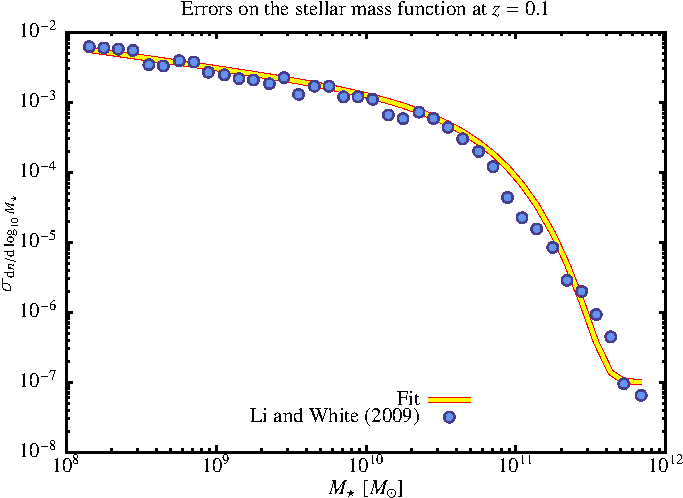
\includegraphics[width=160mm]{../plots/stellarMassFunctionErrors_z01.pdf}
 \end{center}
 \caption{Errors on the \protect\cite{li_distribution_2009} stellar mass funtion (points) and the fitting function (line) given by eqn.~(\protect\ref{eq:stellarMassFunctionErrorsFit}).}
 \label{fig:stellarMassFunctionErrors}
\end{figure}

\begin{figure}
 \begin{center}
 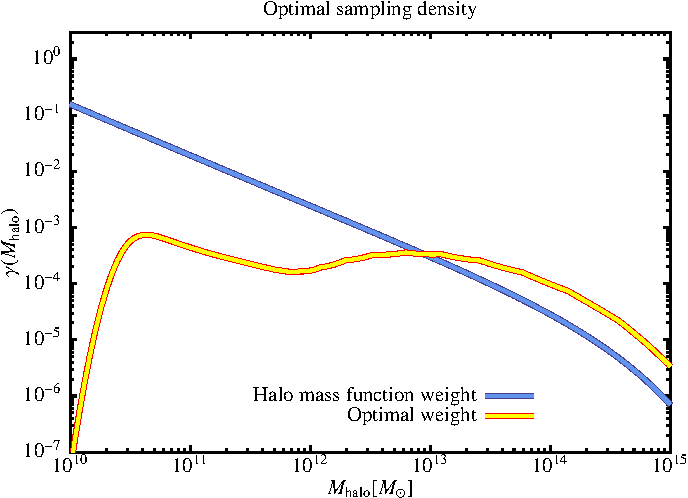
\includegraphics[width=160mm]{../plots/optimalSamplingStellarMassFunction.pdf}
 \end{center}
 \caption{Optimal weighting (yellow line) compared with weighting by the dark matter halo mass function (i.e. sampling halos at random from a representative volume; blue line). Sampling densities have been normalized to unit compute time.}
 \label{fig:optimalSamplingStellarMassFunction}
\end{figure}

\subsection{Refining by Other Merger Tree Statistics}

Since building merger trees is relatively fast, while solving the baryonic physics is slow it may be advantageous to  non-uniformly sample the distribution of merger trees at fixed merger tree mass, $M$. For example, we could assign some measure of formation history to each merger tree, such as the time since the last major merger, $\tau$. The halo mass function then becomes $n(M,\tau)$ (which can be computed by simulating large numbers of trees), and the tree sampling function becomes $\gamma(M,\tau)$. We'd then need to know the stellar mass function conditioned on both $M$ and $\tau$, $\phi_\star(M_\star|M,\tau)$. Given these, the above approach could be easily generalized to determine an optimal $\gamma(M,\tau)$. Then, after generating a merger tree, we'd first compute $\tau$. If a sufficient number of trees in that $\tau$ interval had already been computed, then we'd simply drop that tree and compute another one. The speed up here would depend on how fast building trees is relative to solving baryonic physics and what fraction of trees you discard. In principle, the trees could be generated, sampled and stored in advance so that we'd already have an optimally distributed set of trees in $M$ and $\tau$ that could be used for each model run.

\section{Constraints}\label{sec:ConstraintScripts}

Any constraint which can be applied to \glc\ is defined by two files, a configuration file and a likelihood script, which must be placed in {\tt constraints/constraints} and {\tt constraints/scripts} respectively. 

\subsection{Configuration File}\label{sec:ConstraintConfigFiles}

The configuration file should have the form:
\begin{verbatim}
<!-- Defines a constraint to match some data. -->                                          
<constraint>                                                                                                         
  <name>Long-form name of this constraint</name>                                                                      
  <label>shortLabelForThisConstraint</label>                                                                        
  <outputRedshift>0.07</outputRedshift>                                                                              
  <outputRedshift>1.00</outputRedshift>                                                                              
  <haloMassResolution>5.0e9</haloMassResolution>                                                                     
  <haloMassMinimum>2.0e10</haloMassMinimum>                                                                          
  <haloMassMaximum>2.0e14</haloMassMaximum>                                                                          
  <analysis>constraints/scripts/myAnalysisScript.pl</analysis>                                         
  <luminosity>
    <filter>UKIRT_K</filter>
    <redshift>0.0</redshift>
    <frame>rest</frame>
  </luminosity>
  <luminosity>
    <filter>UKIRT_K</filter>
    <redshift>1.0</redshift>
    <frame>observed</frame>
  </luminosity>
  <optionOn>outputMainBranchStatus</optionOn>
  <optionOn>outputDensityContrastData</optionOn>
  <parameter>
   <name>outputDensityContrastValues</name>
   <value>200.0</value>
   <accumulation>unique</accumulation>
  </parameter>
</constraint>                                                                                                        
\end{verbatim}
The {\tt name} and {\tt label} are used to describe the constraint ({\tt label} is used as a suffix in file names so should not contain spaces or other characters which might cause problems in file names). 

The remaining elements describe the requirements for this constraint. {\tt haloMassResolution} specifies the maximum resolution in mergers trees that still allows this constraint to be computed accurately. Similarly, {\tt haloMassMinimum} and {\tt haloMassMaximum} specify the required range of halo masses to simulate to allow this constraint to be computed accurately.

One or more {\tt outputRedshift} elements may be present, each specifying a redshift at which output is required for this constraint. Similarly, one or more {\tt luminosity} elements may be present, each of which specifies a luminosity which must be computed for this constraint. Each {\tt luminosity} must contain a specification of {\tt filter}, {\tt redshift}, and {\tt frame} to define which luminosity is to be computed.

One or more {\tt optionOn} elements may be present. Each element must specify the name of a \glc\ input parameter. That parameter will be set to {\tt true} in the \glc\ input parameter file.

Finally, arbitrary other parameter may be set using the standard {\tt parameter} element which should give the {\tt name} and {\tt value} for the parameter. Optionally, an {\tt accumulation} element may also be specified for each {\tt parameter}. This controls how values of the parameter are to be accumulated if set by more than one constraint. An accumulation of {\tt overwrite} will simply overwrite any previously set values. An accumulation of {\tt combine} will concatenate all values set by different constraints. Finally, an accumulation of {\tt unique} will concatenate all values set by different constraints and then filter out any duplicates.

When multiple constraints are used, their requirements are automatically combined.

\subsection{Likelihood Script}

The likelihood script for a constraint is required to perform several tasks, controlled by command line options. The script should accept the following command line syntax:
\begin{verbatim}
 myScript.pl <galacticusFile> [options...]
\end{verbatim}
where {\tt galacticusFile} is the file name of the \glc\ model for which the likelihood calculation should be performed. The following options must be supported by the script:
\begin{description}
 \item [{\tt --plotFile <fileName>}] If this option is present, the script should generate a plot showing the constraint and the model result and write it to {\tt fileName}.
 \item [{\tt --outputFile <fileName>}] If this option is present, the script should compute the log-likelihood of the model given the constraint and write it to {\tt fileName} using the format
\begin{verbatim}
 <constraint>
  <logLikelihood>-123</logLikelihood>
 </constraint>
\end{verbatim}
 \item [{\tt --accuracyFile <fileName>}] If this option is present, the script should write an XML file giving details of the accuracy of the model results relative to the observational errors using the format
\begin{verbatim}
 <accuracy>
  <x>...</x>
  .
  .
  .
  <x>...</x>
  <yModel>...</yModel>
  .
  .
  .
  <yModel>...</yModel>
  <yData>...</yData>
  .
  .
  .
  <yData>...</yData>
  <errorModel>...</errorModel>
  .
  .
  .
  <errorModel>...</errorModel>
  <errorData>...</errorData>
  .
  .
  .
  <errorData>...</errorData>
 </accuracy>
\end{verbatim}
In this file the {\tt yModel} and {\tt yData} elements should give the values of the model result and the comparable data respectively, while {\tt errorModel} and {\tt errorData} should give an estimate of the errors on these quantities. In the case of the model error this should include only the contribution arising from the finite number of merger trees simulated. This file will be used to judge whether the model is running sufficient merger trees such that the likelihood is not dominated by these errors. The {\tt x} elements are optional but can be used to give the parameter values associated with each model result.
 \item [{\tt --resultFile <fileName>}] If this option is present, the script should write an XML file giving details of the result of the model using the format
\begin{verbatim}
 <accuracy>
  <x>...</x>
  .
  .
  .
  <x>...</x>
  <y>...</y>
  .
  .
  .
  <y>...</y>
  <error>...</error>
  .
  .
  .
  <error>...</error>
 </accuracy>
\end{verbatim}
In this file the {\tt y} elements should give the values of the model result, while the {\tt error} elements should give an estimate of the errors on these results. The error should include only the contribution arising from the finite number of merger trees simulated. This file will be used to judge whether the model result is converged with respect to various numerical parameters in \glc. The {\tt x} elements are optional but can be used to give the parameter values associated with each model result.
 \item [{\tt --modelDiscrepancies <path>}] If this option is present, the script should scan {\tt path}. For each directory found in {\tt path} the script should check for the existance of a file named {\tt discrepancy<label>.hdf5} where {\tt label} is the label given for this constraint in its configuration file (see \S\ref{sec:ConstraintConfigFiles}). If present, the model discrepancy given in that file should be applied to the likelihood calculation. See \S\ref{sec:ModelDiscrepancy} for a description of the structure of the discrepancy files.
\end{description}

\subsection{Available Constraints}

\subsubsection{Li \& White (2009) SDSS Stellar Mass Function}

This constraint utilizes the stellar mass function for $z\approx 0.07$ galaxies measured by \cite{li_distribution_2009} from the \gls{sdss}. The mass function reported by \cite{li_distribution_2009} is converted to the appropriate Hubble constant for the given \glc\ model (assuming that masses scale as $H_0^{-2}$ and volumes as $H_0^3$)---no adjustment is made for cosmological parameters given the low redshift of the sample.

Given a \glc\ model, total stellar masses of model galaxies are adjusted using:
\begin{equation}
 M_\star \rightarrow {\bf G} {\bf S} M_\star 
\end{equation}
where the ${\bf S}$ operator is a multiplicative factor accounting for systematic errors in stellar mass determination and is equal to \citep{behroozi_comprehensive_2010}
\begin{equation}
 \log_{\rm 10} S = \mu + \kappa \log_{\rm 10} \left({M_\star \over 10^{11.3}M_\odot}\right)
\end{equation}
where $\mu=${\tt [sdssStellarMassFunctionZ0.07StellarMassSystematicMu]}, $\kappa=${\tt [sdssStellarMassFunctionZ0.07StellarMassSystematiKappa]}, and the {\bf G} operator is a multiplicative factor drawn from a log-normal distribution of width $0.07$~dex for each galaxy to mimic the effects of random errors on stellar masses (motivated by the discussion of \cite{behroozi_comprehensive_2010}).

The model masses are then used to construct a mass function by binning into a histogram using the masses reported by \cite{li_distribution_2009} (modified as described above) as the centers of the bins (with bin boundaries placed at the geometric means of consecutive bin centers).

If the {\tt --modelDiscrepancies} option is given, then any multiplicative or additive discrepancies found are applied to the model mass function, and any additional covariance is added to the covariance matrix.

The covariance matrix is computed as
\begin{equation}
 {\bf C} = {\bf C}_{\rm obs} + {\bf C}_{\rm model,random} + \sum_i {\bf C}_{{\rm discrepancy}, i},
\end{equation}
where ${\bf C}_{\rm obs}$ is the covariance matrix of the observational data, ${\bf C}_{\rm model,random}$ is the covariance matrix of the model arising from random noise (due to the finite number of trees simulated, and approximated as a Poisson process for each galaxy, with off-diagonal terms arising because each galaxy contributes a Gaussian distribution to the mass function due to modelling of random errors in stellar mass determinations), and ${\bf C}_{{\rm discrepancy}, i}$ is the covariance due to the $i^{\rm th}$ model discrepancy.

The model likelihood is then computed using:
\begin{equation}
 \mathcal{L} = {1 \over \sqrt{(2 \pi)^n |{\bf C}|}} \exp\left[ -{1\over 2} \Delta {\bf C}^{-1} \Delta \right],
\end{equation}
where $\Delta_i = \Phi_{{\rm model}, i} - \Phi_{{\rm observed}, i}$ is the difference between the model and observed mass functions, and $n$ is the number of points in the mass function histogram.

\section{Constraint Compilations}
